\switchcolumn[1]*
\codeblock{reduction_factors}
\switchcolumn[0]

\subsection{Empirical Risk Minimization}
We consider supervised learning with a neural network $f\colon \gX \times \Theta \to \gF$ that maps a given input $\vx \in \gX$ from a domain $\gX$ to a prediction $f(\vx, \vtheta) \in \gF$ in a prediction space $\gF$ using parameters $\vtheta \in \Theta$ from a parameter space $\Theta$.
Predictions are scored with a criterion function $c\colon \gF \times \gY \to \sR$ that compares the prediction to the true target $\vy \in \gY$ from a label space $\gY$, producing a single number called the loss on datum $(\vx, \vy)$.

For a data set $\sD = \{(\vx_n, \vy_n) \mid n=1, \dots, N\}$ of collected labelled examples, we evaluate the per-datum criteria and accumulate them into the total loss, using an accumulation factor $R \in \sR$,
\begin{align}\label{eq:empirical_risk}
  \begin{split}
    \gL_{\sD}(\vtheta) & = R \sum_{n=1}^N \ell_n(\vtheta)
    \\
                       & = R \sum_{n=1}^N c(f(\vx_n, \vtheta), \vy_n)\,.
  \end{split}
\end{align}
Common choices for $R$ are $\nicefrac{1}{N}, 1, \nicefrac{1}{N \dim(\gY)}$; see \Cref{basics/reduction_factors} for a function that computes $R$.
The goal of training is to find the parameters $\vtheta$ that reduce the empirical risk $\gL_{\sD}(\vtheta)$ without overfitting to the training data.

\Cref{eq:empirical_risk} disentangles `the loss' into three components: the neural network $f$, the criterion function $c$, and the reduction factor $R$.
The most common loss functions are the square loss for regression and the softmax cross-entropy loss for classification.
We show their criterion and reduction factors in \cref{ex:square_loss,ex:cross_entropy_loss}).

\switchcolumn[1]
\begin{example}[Square loss, \Cref{basics/reduction_factors}]\label{ex:square_loss}
  For least squares regression with vector-valued targets ($\gY = \sR^C = \gF$), the criterion and reduction factor of PyTorch's \texttt{nn.MSELoss} are
  \begin{align*}
    &c(\vf, \vy)
      =
      \frac{1}{2}\sum_{c=1}^C [\vf - \vy]_c^2\,,
    \\
    R
    &=
      \begin{cases}
        2                     & \text{\texttt{reduction="sum"}}
        \\
        \frac{2}{N \dim(\gY)} & \text{\texttt{reduction="mean"}}
      \end{cases}
  \end{align*}
  where $\dim(\gY) = C$ in the vector case, but $\gY = \gF$ could also be a matrix or tensor space.
\end{example}

\begin{example}[Cross-entropy loss, \Cref{basics/reduction_factors}]\label{ex:cross_entropy_loss}
  For classification, with categorical targets ($\gY = \{1, \dots, C\}$ and $\gF = \sR^C$), PyTorch's \texttt{nn.CrossEntropyLoss} uses the following criterion function and reduction factor
  \begin{align*}
    &c(\vf, y)
      =
      - \log([\softmax(\vf)]_y)\,,
    \\
    R
    &=
      \begin{cases}
        1                     & \text{\texttt{reduction="sum"}}
        \\
        \frac{1}{N \dim(\gY)} & \text{\texttt{reduction="mean"}}
      \end{cases}
  \end{align*}
  with $[\softmax(\vf)]_i = \nicefrac{\exp([\vf]_i)}{\sum_{j=1}^C \exp([\vf]_{j})}$.
  For the vector case $\dim(\gY) = 1$, but $\gY, \gF$ could also be compatible matrix or tensor spaces in a more general setup where we aim to classify sequences of categorical labels.
\end{example}
\switchcolumn[0]

\begin{caveat}[Scaling]
  Implementations of loss functions mix the concepts of criterion and reduction.
  This is often fine, but sometimes makes it difficult to translate to new loss functions without accidentally forgetting a factor.
  By keeping both concepts separate, we reduce the chance of introducing scaling bugs.
\end{caveat}

%%% Local Variables:
%%% mode: latex
%%% TeX-master: "../main"
%%% End:


\switchcolumn[1]*
\codeblock{forward_pass}
\switchcolumn[0]

\subsection{Deep neural networks}
We consider sequential neural networks as they are simple and widely used.
They are composed of $L$ layers $f^{(l)}(\cdot, \vtheta^{(l)}), l=1,\dots, L$, each of which can have its own parameters $\vtheta^{(l)}$.
The whole network is simply a stack of layers, \ie $f = f^{(L)} \circ \dots \circ f^{(1)}$, and the evaluation produces a set of intermediate features,
\begin{align*}
  \vx^{(l)} = f^{(l)}(\vx^{(l-1)}, \vtheta^{(l)}), \quad l=1,\dots, L,
\end{align*}
starting with $\vx^{(0)} \leftarrow \vx$, ending in $\vx^{(L)} \leftarrow f(\vx, \vtheta)$.
We refer to the hidden representations $\vx^{(l-1)}$ as the \emph{input to layer $l$}, and to $\vx^{(l)}$ as the \emph{output of layer $l$}.
Some layers have empty parameters, e.g.\,activation, pooling, or dropout layers.

To compute KFAC, we will need access to the inputs and outputs of certain layers.
We can obtain these by intercepting the neural net's forward pass using PyTorch's hook mechanism, see \Cref{basics/forward_pass}.
%%% Local Variables:
%%% mode: latex
%%% TeX-master: "../main"
%%% End:


\subsection{Probabilistic interpretation}
So far, we have considered minimizing an empirical risk over a data set given an arbitrary criterion function $c$.
Now, we take a step back and first describe empirical risk minimization as an approximation of minimizing the intractable population risk.
This perspective connects to a probabilistic interpretation of empirical risk minimization as maximum likelihood estimation that will occur throughout the tutorial, \eg when we define the Fisher information matrix as curvature matrix (\cref{subsec:curvature-matrices}).

\paragraph{Empirical risk as expectation.} Recall the empirical risk from \cref{eq:empirical_risk} which we minimize during training,
\begin{align*}
  \min_{\vtheta} \gL_{\sD}(\vtheta) = \min_{\vtheta} R \sum_{n=1}^N \ell_n(\vtheta)\,.
\end{align*}
Why is it called an `empirical' risk?
Because it can be expressed as expectation over an empirical distribution in the following sense:

Assume there exists a data-generating process $p_{\text{data}}(\rvx, \rvy)$ over input-target pairs.
Ideally, we want to minimize the risk over this distribution,
\begin{align*}
  \argmin_{\vtheta} \E_{(\vx, \vy) \sim p_{\text{data}}(\rvx, \rvy)}[c(f(\vx, \vtheta), \vy)]\,.
\end{align*}
However, $p_{\text{data}}$ is intractable.
Therefore, we draw a finite collection of samples into a data set
\begin{align*}
  \sD = \{ (\vx_n, \vy_n) \mid (\vx_n, \vy_n) \stackrel{\text{\iid}}{\sim} p_{\text{data}}(\vx, \vy) \}\,.
\end{align*}
Then, we can replace the intractable data-generating process $p_{\text{data}}$ with the tractable empirical distribution $p_{\sD}(\rvx, \rvy)$ implied by data set $\sD$.
It consists of a uniformly weighted sum of delta peaks around the collected data points,
\begin{align*}
  p_{\sD}(\rvx, \rvy) = \frac{1}{N} \sum_{n=1}^N \delta(\rvx - \vx_n) \delta(\rvy - \vy_n)\,.
\end{align*}
This turns risk minimization into a tractable task:
\begin{align*}
  & \argmin_{\vtheta} \E_{(\vx, \vy) \sim \colored{p_{\text{data}}(\rvx, \rvy)}}[c(f(\vx, \vtheta), \vy)]
  \\
  \approx & \argmin_{\vtheta} \E_{(\vx, \vy) \sim \colored{p_{\sD}(\rvx, \rvy)}}[c(f(\vx, \vtheta), \vy)].
  \\
  \intertext{By writing out the expectation, we obtain}
  =       & \argmin_{\vtheta} \frac{1}{N} \sum_n c(f(\vx_n, \vtheta), \vy_n).
  \\
  \intertext{Note that the minimized objective is the empirical risk in \cref{eq:empirical_risk}
  scaled by $\nicefrac{1}{NR}$.
  However, we can arbitrarily scale objectives without changing the
  location of their minima.
  Hence, the above is equivalent to minimizing the empirical risk
  }
  =& \argmin_{\vtheta} \gL_{\sD}(\vtheta)\,.
\end{align*}
We have thus shown that empirical risk minimization is minimizing a (scaled) expectation of the criterion $c$ over an empirical density $p_{\sD}(\rvx, \rvy)$.

\paragraph{The neural net parameterizes a likelihood.}
Let's approach this from a probabilistic perspective now.
Assume we want to learn $p_{\text{data}}(\rvx, \rvy) = p_{\text{data}}(\rvy \mid \rvx) p_{\text{data}}(\vx)$ using a parameterized density of the form $p(\rvx, \rvy \mid \vtheta) = p(\rvy \mid \rvx, \vtheta) p_{\text{data}}(\rvx)$ where $p_{\text{data}}(\rvx) = \int p_{\text{data}}(\rvx, \rvy)\ \mathrm{d}\rvy$ is the marginal density of the input data.
Note that we only model the likelihood of the labels with parameters $\vtheta$.

One plausible approach to make $p$ resemble $p_{\text{data}}$ is to minimize their KL divergence,
\begin{align*}
  & \argmin_{\vtheta} \mathrm{KL}(p_{\text{data}}(\rvx, \rvy) \mid\mid p(\rvx, \rvy \mid \vtheta))\,.
  \\
  \intertext{We can simplify this expression by substituting the definition of the KL divergence and dropping terms that do not depend on $\vtheta$,}
  \Leftrightarrow & \argmin_{\vtheta} \E_{p_{\text{data}}(\rvx, \rvy)}[- \log( p(\rvx, \rvy \mid \vtheta))]\,.
  \\
  \intertext{This looks very similar to the expected risk from above.
  Next, let's factorize our model distribution using its conditional and marginal densities and drop $p_{\text{data}}(\rvx)$ as it does not depend on $\vtheta$,
  }
  \Leftrightarrow & \argmin_{\vtheta} \E_{p_{\text{data}}(\rvx, \rvy)}[- \log( p(\rvy \mid \rvx, \vtheta))]\,.
                    \intertext{To make this problem tractable, we need to replace the intractable data-generating process $p_{\text{data}}(\rvx, \rvy)$ with the empirical distribution $p_{\sD}(\rvx, \rvy)$ again:}
                    \approx         & \argmin_{\vtheta} \E_{p_{\sD}(\rvx, \rvy)}[- \log( p(\rvy \mid \rvx, \vtheta))].
  \\
  \intertext{Writing out the expectation, we obtain}
  =               & \argmin_{\vtheta} \frac{1}{N} \sum_n - \log( p(\rvy = \vy_n \mid \rvx=\vx_n,\vtheta)).
  \\
  \intertext{To make this expression more similar to the empirical risk, we introduce a general scaling $R$ and change the likelihood's parameterization from $p(\rvy \mid \rvx, \vtheta)$ to $r(\rvy \mid f(\rvx, \vtheta))$ with a neural net $f$:}
  =               & \argmin_{\vtheta} R \sum_n - \log( r(\rvy = \vy_n \mid f(\vx_n,\vtheta)))
\end{align*}
This parameterization makes it clear that the neural network represents a conditional distribution over the labels given the inputs (and parameters).

\paragraph{The criterion is the negative log-likelihood.}
We are now very close to writing down the explicit connection between empirical risk minimization and maximum likelihood estimation.
The last remaining step is to connect the model's likelihood $r(\rvy \mid f(\rvx, \vtheta))$ with the criterion function $c(f(\vx, \vtheta), \vy)$ from empirical risk minimization.
It turns out that empirical risk minimization with square loss (\cref{ex:square_loss}) corresponds to maximum likelihood estimation (or equivalently, negative log-likelihood minimization) of a Gaussian distribution over the labels (\cref{ex:square_loss_probabilistic}).
Similarly, classification with softmax cross-entropy criterion amounts to maximum likelihood estimation where the neural net parameterizes a categorical distribution (\cref{ex:cross_entropy_loss_probabilistic}).
\Cref{basics/label_sampling} provides functions to sample labels from these distributions.

The neural net's interpretation as a likelihood allows using probabilistic concepts to measure similarity for comparing two networks.
This will be useful when we define the Fisher information matrix (\cref{sec:fisher}), a common curvature matrix.

\switchcolumn[1]
\begin{example}[Probabilistic interpretation of the square loss]\label{ex:square_loss_probabilistic}
  For the square loss from \Cref{ex:square_loss}, we have that $c(\vf, \vy) = - \log( \mathrm{const.}
  \cdot \gN(\rvy \mid \vmu = f(\vx, \vtheta), \mSigma = \mI))$ where $\gN(\bullet \mid \vmu, \mSigma)$ is a multivariate Gaussian distribution with mean $\vmu \in \sR^C$ and positive definite covariance $\mSigma \in \sR^{C \times C}$,
  \begin{align*}
    \gN(\rvy \mid \vmu, \mSigma)
    =
    \frac{
    \exp\left( -\frac{1}{2} {(\rvy - \vmu)}^\top \mSigma^{-1} (\rvy - \vmu) \right)
    }{{(2\pi)}^{C/2} \sqrt{\det(\mSigma)}}\,.
  \end{align*}
  We can safely neglect the constant factor for the optimization problem and, by setting the covariance to the identity matrix and the mean to the neural net's prediction, identify that empirical risk minimization with square loss corresponds to maximum likelihood estimation of a Gaussian likelihood with unit covariance and mean parameterized by the network:
  \begin{align*}
    c                             & = \text{\texttt{MSELoss}}
    \\
                                  & \Leftrightarrow
    \\
    r(\rvy \mid f(\rvx, \vtheta)) & = \gN(\rvy \mid \vmu = f(\vx, \vtheta), \mSigma = \mI)\,
    \\
                                  & \Leftrightarrow
    \\
    p(\rvy \mid \rvx, \vtheta)    & = \gN(\rvy \mid \vmu = f(\vx, \vtheta), \mSigma = \mI)\,.
  \end{align*}
\end{example}

\begin{example}[Probabilistic interpretation of cross-entropy loss]\label{ex:cross_entropy_loss_probabilistic}
  For cross-entropy loss from \Cref{ex:cross_entropy_loss}, we have that $c(\vf, y) = - \log( \gC(\ry \mid \vsigma = \softmax(\vf) ))$ where $\gC(\bullet \mid \vsigma)$ is a categorical distribution over $\{1, \dots, C\}$ with probabilities $\vsigma \in \sR^C_{\ge 0}$ and $\vsigma^\top \vone = 1$,
  \begin{align*}
    \gC(\ry \mid \vsigma)
    =
    \prod_{c=1}^C [\vsigma]_c^{\delta_{\ry,c}}\,.
  \end{align*}
  Hence, we can identify that empirical risk minimization with softmax cross-entropy loss amounts to maximum likelihood estimation with a categorical likelihood parameterized by the softmax of the network's output:
  \begin{align*}
    c                             & = \text{\texttt{CrossEntropyLoss}}
    \\
                                  & \Leftrightarrow
    \\
    r(\ry \mid f(\rvx, \vtheta)) & = \gC(\ry \mid \vsigma = \softmax(f(\vx, \vtheta)))\,
    \\
                                  & \Leftrightarrow
    \\
    p(\ry \mid \rvx, \vtheta)    & = \gC(\ry \mid \vsigma = \softmax(f(\vx, \vtheta)))\,.
  \end{align*}
\end{example}

\codeblock{basics/label_sampling}
\switchcolumn[0]
%%% Local Variables:
%%% mode: latex
%%% TeX-master: "../main"
%%% End:


\subsection{Derivatives \& Automatic Differentiation}

\begin{caveat}
  In deep learning, we often work with matrices, or higher-dimensional tensors.
  We want to use matrix linear algebra expressions to avoid using heavy index notation.
  This can be achieved by flattening all tensors back into vectors and re-using definitions derivatives from the vector case.
  However, we must be careful when translating the results back to the tensor format, as the translation process depends on the flattening convention.
  Classically, the mathematical derivations prefer a \emph{different} flattening scheme than the one used in deep learning libraries.
\end{caveat}

\switchcolumn[0]*
\subsubsection{Flattening}
There are many ways to flatten the entries of a tensor into a vector.
The two by far most common conventions are (i) last-varies-fastest ($\cvec$) and (ii) first-varies-fastest ($\rvec$).
Their names are easy to remember from their action on a matrix (see \Cref{ex:flattening}): $\cvec$-flattening concatenates columns into a vector (column flattening); $\rvec$-flattening concatenates rows into a vector (row flattening).
Column-flattening is popular in mathematical presentations, while row-flattening is popular in deep learning libraries which lay out tensors in row-major format in memory.
To see their differences, we will implement both.

For arbitrary tensors, we can generalize the matrix flattenings by ordering entries such that either their last index ($\cvec$, \Cref{def:cvec}) or first index ($\rvec$, \Cref{def:rvec}) varies fastest:

\switchcolumn[1]*
\codeblock{basics/flattening}
\switchcolumn[0]

\begin{setup}\label{setup:flattening}
  Let $\tA \in \sR^{N_1 \times \dots \times N_A}$ be a tensor of rank $A$ whose entries are indexed through a tuple $(n_1, \dots, n_A)$ where $n_a \in \{1, \dots, N_a\}$.
\end{setup}
\begin{definition}[$\cvec$, \Cref{flattening}]\label{def:cvec}
  The first-varies-fastest flattening of $\tA$ from \Cref{setup:flattening} is
  \begin{align*}
    \cvec(\tA) =
    \begin{pmatrix}
      \etA_{1,1,\dots,1} \\
      \etA_{2,1,\dots,1} \\
      \vdots \\
      \etA_{N_1,1,\dots,1} \\
      \etA_{1,2,\dots,1} \\
      \vdots \\
      \etA_{N_1,2,\dots,1} \\
      \vdots \\
      \etA_{N_1,N_2,\dots,N_A}
    \end{pmatrix}
    \in \sR ^{N_1 \cdots N_A}\,.
  \end{align*}
\end{definition}

\begin{definition}[$\rvec$, \Cref{flattening}]\label{def:rvec}
  The last-varies-fastest flattening of $\tA$ from \Cref{setup:flattening} is
  \begin{align*}
    \rvec(\tA) =
    \begin{pmatrix}
      \etA_{1,\dots,1,1} \\
      \etA_{1,\dots,1,2} \\
      \vdots \\
      \etA_{1,\dots,1,N_A} \\
      \etA_{1,\dots,2,1} \\
      \vdots \\
      \etA_{1,\dots,2,N_A} \\
      \vdots \\
      \etA_{N_1,\dots,N_{A-1},N_A}
    \end{pmatrix}
    \in \sR ^{N_A \cdots N_1}\,.
  \end{align*}
\end{definition}

In code, we will sometimes require partial flattening of a sub-set of contiguous indices, instead of all indices.
The definitions are analogous, but the flattened indices are surrounded by static ones.

\begin{example}[Matrix flattening, \Cref{flattening}]\label{ex:flattening}
  For a matrix
  \begin{equation*}
    \mA = \begin{pmatrix} 1 & 2 \\ 3 & 4 \end{pmatrix}
  \end{equation*}
  we have
  \begin{equation*}
    \rvec(\mA)
    =
    \begin{pmatrix}
      1 \\ 2 \\ 3 \\ 4
    \end{pmatrix}\,,
    \qquad
    \cvec(\mA)
    =
    \begin{pmatrix}
      1 \\ 3 \\ 2 \\ 4
    \end{pmatrix}\,.
  \end{equation*}
\end{example}
%%% Local Variables:
%%% mode: latex
%%% TeX-master: "../main"
%%% End:


\switchcolumn[0]*
\subsubsection{Jacobians, JVP, VJPs}
Building up to curvature approximations that tackle the approximation of second-order partial derivatives, we start with first-order derivatives.
These are collected into a matrix called the Jacobian, which depends on the flattening convention.
We can multiply with the Jacobian and its transpose via automatic differentiation, without building up the matrix in memory.
These operations are called vector-Jacobian products (VJPs) and Jacobian-vector products (JVPs), respectively.

Machine learning libraries like JAX and PyTorch offer routines for computing Jacobians, VJPs, and JVPs.
However, their interface is functional.
Here, we provide an alternative implementation that accepts nodes of a computation graph rather than functions as input and will be beneficial for modular implementations of neural networks, as we consider later.
We also provide examples for important Jacobians, namely the output-parameter Jacobian of an affine map, \ie a linear layer.
These Jacobians exhibit Kronecker structure, which is the foundation for the `K' in KFAC.
We verify this structure numerically and observe how the flattening convention affects it.

\begin{setup}[Vector-to-vector function]\label{setup:vector_to_vector_function}
  Let function $f: \sR^A \to \sR^B, \va \mapsto \vb = f(\va)$ denote a vector-to-vector function.
\end{setup}

\begin{definition}[Jacobian of a vector-to-vector function]\label{def:vector_jacobian}
  The Jacobian of a vector-to-vector function $f$ from \Cref{setup:vector_to_vector_function}, $\jac_{\va}\vb \in \sR^{B \times A}$, collects the first-order partial derivatives into a matrix such that
  \begin{align*}
    [\jac_{\va} \vb]_{i,j} = \frac{\partial [f(\va)]_i}{\partial [\va]_j}\,.
  \end{align*}
\end{definition}
\Cref{def:vector_jacobian} is limited to vector-to-vector functions.
The more general Jacobian of a tensor-to-tensor function can be indexed with combined indices from the input and output domains:

\begin{setup}[Tensor-to-tensor function]\label{setup:jacobians}
  Consider a tensor-to-tensor function $f: \sR^{A_1 \times \dots \times A_N} \to \sR^{B_1 \times \dots \times B_M}, \tA \mapsto \tB = f(\tA)$ from a rank-$N$ tensor $\tA$ into a rank-$M$ tensor $\tB$.
\end{setup}

\begin{definition}[General Jacobian, \Cref{basics/jacobians}]\label{def:general_jacobian}
  The general Jacobian of $f$ from \Cref{setup:jacobians}, $\tJ_{\tB}\tA$, is a rank-$(M+N)$ tensor that collects the first-order partial derivatives such that
  \begin{align*}
    [\tJ_{\tA}\tB]_{\colored{i_1, \dots, i_M}, \colored[VectorPink]{j_1, \dots, j_N}}
    =
    \frac{\partial [f(\tA)]_{\colored{i_1, \dots, i_M}}}{\partial [\tA]_{\colored[VectorPink]{j_1, \dots, j_N}}}\,.
  \end{align*}
\end{definition}
For $M=N=1$, the general Jacobian reduces to the Jacobian of a vector-to-vector function from \Cref{def:vector_jacobian}.

\switchcolumn[1]*
\codeblock{basics/jacobian_products}
\switchcolumn[0]

\paragraph{Jacobian multiplication.} In practice, this general Jacobian can be prohibitively large and therefore one must almost always work with it in a matrix-free fashion, \ie through VJPs and JVPs.

\begin{definition}[Vector-Jacobian products (VJPs), \Cref{basics/jacobian_products}]\label{def:vjp}
  Given a tensor-to-tensor function $f$ from \Cref{setup:jacobians} and a tensor $\tV \in \sR^{B_1 \times \dots \times B_M}$ in the output domain, the vector-Jacobian product (VJP) $\tU$ of $\tV$ and $\tJ_{\tA}\tB$ lives in $f$'s input domain and follows by contracting the \colored{output indices},
  \begin{align*}
    & [\tU]_{j_1, \dots, j_N}
    \\
    & =
      \colored{\sum_{i_1, \dots, i_M}}
      [\tV]_{\colored{i_1, \dots, i_M}}
      [\tJ_{\tA}\tB]_{\colored{i_1, \dots, i_M}, j_1, \dots, j_N}\,.
  \end{align*}
\end{definition}
For $M=N=1$, $\tV, \tU \to \vv, \vu$ are column vectors, $\tJ_{\tA}\tB \to \jac_{\va}\vb$ is a matrix, and the VJP is $\vu^{\top} = \vv^{\top} (\jac_{\va}\vb)$ or $\vu = (\jac_{\va}\vb)^{\top} \vv$, \ie multiplication with the transpose Jacobian.

VJPs are at the heart of reverse-mode automatic differentiation, aka backpropagation (this is why $\tU$ is often called the \emph{pull-back} or \emph{backpropagation} of $\tV$ through $f$).
Therefore, they are easy to implement with standard functionality (\eg \texttt{autograd.grad} in PyTorch).

The other relevant contraction is between the Jacobian and a vector from the input domain:

\begin{definition}[Jacobian-vector products (JVPs), \Cref{basics/jacobian_products}]\label{def:jvp}
  Given a tensor-to-tensor function $f$ from \Cref{setup:jacobians} and a tensor $\tV \in \sR^{A_1 \times \dots \times A_N}$ in the input domain, the Jacobian-vector product (JVP) $\tU$ between $\tV$ and $\tJ_{\tA}\tB$ lives in $f$'s output domain and follows by contracting the \colored[VectorPink]{input indices},
  \begin{align*}
    & [\tU]_{j_1, \dots, j_M}
    \\
    & =
      \colored[VectorPink]{\sum_{i_1, \dots, i_N}}
      [\tJ_{\tA}\tB]_{j_1, \dots, j_M, \colored[VectorPink]{i_1, \dots, i_N}}
      [\tV]_{\colored[VectorPink]{i_1, \dots, i_N}}\,.
  \end{align*}
\end{definition}
For the vector case, $\tU, \tV, \tJ_{\tA}\tB \to \vu, \vv, \jac_{\va}\vb$, the JVP is $\vu = (\jac_{\va}\vb) \vv$, as suggested by its name.
JVPs are common in forward-mode automatic differentiation ($\tU$ is often called the \emph{pushforward} of $\tV$ through $f$).
Only recently has this mode garnered attention.
The current JVP functionality in ML libraries usually follows a functional API.
To obtain an implementation that accepts variables from a computation graph and is more compatible with the modular approach we chose in this tutorial, we can use a trick that implements a JVP using two VJPs \cite{townsend2017new}.

\switchcolumn[1]*
\begin{figure}[!h]
  \centering
  \begin{tikzpicture}[%
    % font=\scriptsize,%
    thick,
    box/.style = {rectangle, draw=black, rounded corners, fill=VectorGray!50},%%
    ]
    \node[box] (A) at (0,0) {$f: \tA \mapsto \tB = f(\tA)$};
    \node[box] (B) at (5.5,0) {$\jac_{\tA}\tB$};
    \node[box, align=center] (C) at (0,-3) {%
      $f^{\vec} = \vec \circ f \circ \vec^{-1}$\\%
      $\vec(\tA) \coloneq \va \mapsto \vec(\tB) \coloneq \vb$%
    };
    \node[box, align=center] (D) at (5.5,-3) {%
      $\jac_{\va} \vb$\\%
      $=$\\%
      $\mat(\tJ_{\tA}\tB)$\\%
      $\coloneq$\\%
      $\jac^{\vec}_{\tA}\tB$%
    };
    \draw[-Stealth] (A.east) -- node[fill=white] {$\tJ$} (B.west);
    \draw[-Stealth] (A.south) -- node[fill=white] {flatten $f$} (C.north);
    \draw[-Stealth] (C.east) -- node[fill=white] {$\jac$} (D.west);
    \draw[-Stealth] (B.south) -- node[fill=white] {matricize $\jac_{\tA}\tB$} (D.north);
  \end{tikzpicture}
  \caption{\textbf{Flattening and taking the Jacobian commute and lead to the same matricized Jacobian.}
    $\vec$ denotes one of the flattening conventions from \Cref{def:cvec,def:rvec}.
    $\mat$ denotes matricization (two partial flattenings for row and column dimensions, respectively).}\label{fig:commutative-diagram-jacobian}
\end{figure}
\switchcolumn[0]

\paragraph{Matricization.}
Jacobian products are efficient, but somewhat abstract to work with, as we cannot `touch' the full tensor.
Often, we would also like to think about this tensor as a matrix to be able to present derivations in linear algebra notation.

We can reduce the general Jacobian tensor back to the Jacobian matrix in two different ways: We can either (i) directly matricize the tensor, or (ii) `flatten' the function $f \to f^{\vec}$ such that it consumes and produces vectors, then compute its Jacobian.
Both ways and their resulting Jacobian matrices depend on the flattening convention we choose.
The following definitions are consistent in the sense that both of the aforementioned approaches yield the same result, illustrated by this commutative diagram in \cref{fig:commutative-diagram-jacobian}.


\switchcolumn[1]
\codeblock{basics/jacobians}
\switchcolumn[0]

For this tutorial, the two matrices of interest are the $\cvec$- and $\rvec$-Jacobians.
The $\cvec$-Jacobian is used in mathematical derivations in the literature.
The $\rvec$-Jacobian is common in code.

\begin{definition}[$\cvec$-Jacobian, \Cref{basics/jacobians}]\label{def:cvec_jacobian}
  For a tensor-to-tensor function $f$ from \Cref{setup:jacobians}, its $\cvec$-Jacobian $\jac^{\cvec}_{\tA}\tB \in \sR^{A_N \cdots A_1 \times B_M \cdots B_1}$ is attained by flattening the input and output tensors with $\cvec$ and applying the Jacobian definition for vectors,
  \begin{align*}
    [\jac^{\cvec}_{\tA}\tB]_{i,j}
    =
    \frac{\partial [\cvec(f(\tA))]_i}{\partial [\cvec(\tA)]_j}\,.
  \end{align*}
\end{definition}

\begin{definition}[$\rvec$-Jacobian, \Cref{basics/jacobians}]\label{def:rvec_jacobian}
  For a tensor-to-tensor function $f$ from \Cref{setup:jacobians}, its $\rvec$-Jacobian $\jac^{\rvec}_{\tA}\tB \in \sR^{A_1 \cdots A_N \times B_1 \cdots B_M}$ is attained by flattening the input and output tensors with $\rvec$ and applying the Jacobian definition for vectors,
  \begin{align*}
    [\jac^{\rvec}_{\tA}\tB]_{i,j}
    =
    \frac{\partial [\rvec(f(\tA))]_i}{\partial [\rvec(\tA)]_j}\,.
  \end{align*}
\end{definition}

\paragraph{Example.} The two Jacobians usually differ from each other, albeit in subtle ways.
We highlight their differences on a linear layer, which will be useful later on when we discuss KFAC (\Cref{ex:linear_layer_jacobians}, numerically verified in \cref{basics/jacobians_linear_layer}).
This example reveals two insights:
\begin{itemize}
\item There is a Kronecker structure in the linear layers' Jacobian \wrt its weight.
  This structure is the foundation for the `K' in KFAC.

\item The order of Kronecker factors is reversed depending on the flattening scheme.
  Therefore, we need to be careful when translating results from one convention to the other.
\end{itemize}

\switchcolumn[1]
\begin{example}[$\cvec$- and $\rvec$-Jacobians of a linear layer \wrt its weights, \Cref{basics/jacobians_linear_layer}]\label{ex:linear_layer_jacobians}
  Consider an affine map with weight matrix $\mW \in \sR^{D_{\text{out}} \times D_{\text{in}}}$, bias vector $\vb \in \sR^{D_{\text{out}}}$, input vector $\vx \in \sR^{D_{\text{in}}}$ and output vector $\vz \in \sR^{D_{\text{out}}}$,
  \begin{align*}
    \vz
    \coloneqq
    \mW \vx + \vb
    =
    \begin{pmatrix}
      \mW & \vb
    \end{pmatrix}
    \begin{pmatrix}
      \vx \\ 1
    \end{pmatrix}
    \coloneqq
    \tilde{\mW}
    \tilde{\vx}\,.
  \end{align*}
  To express this operation as matrix-vector multiplication, we combine weight and bias into a single matrix $\tilde{\mW}$ and augment the input with a one, yielding $\tilde{\vx}$, to account for the bias contribution.

  The linear layer's $\cvec$-Jacobian \wrt the combined weight is
  \begin{align*}
    \jac^{\cvec}_{\tilde{\mW}}\vz
    =
    \tilde{\vx}^{\top}
    \otimes
    \mI_{D_{\text{out}}}\,.
  \end{align*}
  In contrast, the $\rvec$-Jacobian is
  \begin{align*}
    \jac^{\rvec}_{\tilde{\mW}}\vz
    =
    \mI_{D_{\text{out}}}
    \otimes
    \tilde{\vx}^{\top}\,,
  \end{align*}
  see \Cref{basics/jacobians_linear_layer}.
  Note that the order of Kronecker factors is \emph{reversed}, depending on the flattening scheme.
\end{example}
\switchcolumn[0]

\switchcolumn[1]
\codeblock{basics/jacobians_linear_layer}
\switchcolumn[0]


% NOTE This example is about weight sharing, which will not be part of the tutorial's
% first version.
\begin{comment}
  \begin{example}[$\cvec$- and $\rvec$-weight Jacobians of a linear layer with weight sharing]
    Consider the same affine map from above, but now processing multiple input vectors $\mX = \begin{pmatrix}\vx_1 & \dots & \vx_S\end{pmatrix} \in \sR^{D_{\text{in}}\times S}$, yielding a sequence $\mZ = \begin{pmatrix} \vz_1 & \dots & \vz_S\end{pmatrix} \in \sR^{D_{\text{out}}\times S}$ where each $\vz_s$ is produced like above.
    The parameters are \emph{shared} over all vectors in the input sequence.
    In matrix notation,
    \begin{align*}
      \mZ
      & \coloneqq
        \mW \mX + \vb \vone^{\top}_S
      \\
      & =
        \begin{pmatrix}
          \mW & \vb
        \end{pmatrix}
        \begin{pmatrix}
          \mX \\ \vone^{\top}_S
        \end{pmatrix}
        \coloneqq
        \tilde{\mW}
        \tilde{\mX}\,.
    \end{align*}
    The $\cvec$-Jacobian \wrt the combined weight is
    \begin{align*}
      \jac^{\cvec}_{\tilde{\mW}}\mZ
      =
      \tilde{\mX}^{\top}
      \otimes
      \mI_{D_{\text{out}}}\,.
    \end{align*}
    In contrast, the $\rvec$-Jacobian is
    \begin{align*}
      \jac^{\rvec}_{\tilde{\mW}}\mZ
      =
      \mI_{D_{\text{out}}}
      \otimes
      \tilde{\mX}^{\top}\,.
    \end{align*}
  \end{example}

  \switchcolumn[1]
  \codeblock{basics/jacobians_shared_linear_layer}
\end{comment}

%%% Local Variables:
%%% mode: latex
%%% TeX-master: "../main"
%%% End:


\switchcolumn[0]*
\subsubsection{Hessians, HVPs}
Now that we have covered first-order derivatives, let's move on to second-order derivatives and develop the necessary concepts to understand KFAC, as well as their implementation.
Second-order derivatives are collected into an object called \emph{the Hessian}.
For our purposes, it will be sufficient to consider the Hessian of functions producing a scalar-valued output.
Let's start with the definition of the Hessian of a vector-to-scalar function.

\begin{setup}[Vector-to-scalar function]\label{setup:vector_to_scalar_function}
  Let $\vf: \sR^A \to \sR, \va \mapsto b = f(\va)$ be a vector-to-scalar function.
\end{setup}

\begin{definition}[Hessian of a vector-to-scalar function]\label{def:vector_hessian}
  The Hessian of a vector-to-scalar function $f$ from \Cref{setup:vector_to_scalar_function} is a matrix $\hess_{\va}b \in \sR^{A \times A}$ collecting the second-order partial derivatives of $f$ into a matrix with
  \begin{align*}
    [\hess_{\va}b]_{i,j}
     & =
    \frac{\partial^2 b}{\partial [\va]_i \partial [\va]_j}\,.
  \end{align*}
\end{definition}
This definition is limited to functions with vector-valued arguments. The extension to tensor-to-scalar functions is straightforward; however, it yields a tensor that is less convenient to work with in terms of notation:

\begin{setup}[Tensor-to-scalar function]\label{setup:hessians}
  Consider a tensor-to-scalar function $f: \sR^{A_1 \times \dots \times A_N} \to \sR, \tA \mapsto b = f(\tA)$ from a rank-$N$ tensor $\tA$ into a scalar $b$.
\end{setup}

\begin{definition}[General Hessian of a tensor-to-scalar function, \Cref{basics/hessians}]\label{def:general_hessian}
  The general Hessian of $f$ from \Cref{setup:hessians}, $\tH_{\tA}b \in \sR^{A_1 \times \dots \times A_N \times A_1 \times \dots \times A_N}$, collects the second-order partial derivatives of $f$ into a tensor with
  \begin{align*}
     & [\tH_{\tA}b]_{\colored{i_1, \dots, i_N}, \colored[VectorPink]{j_1, \dots, j_N}}
    \\
     & =
    \frac{\partial^2 b}{\partial [\tA]_{\colored{i_1, \dots, i_N}} \partial [\tA]_{\colored[VectorPink]{j_1, \dots, j_N}}}\,.
  \end{align*}
\end{definition}

\switchcolumn[1]*
\codeblock{basics/hessian_product}
\switchcolumn[0]

\paragraph{Hessian multiplication.}
Just like for Jacobians, the Hessian tensor is usually too large to be stored in memory.
Hence, one usually works with it implicitly through matrix-vector products, which can be done without computing the Hessian:

\begin{definition}[Hessian-vector products (HVPs), \Cref{basics/hessian_product}]\label{def:hvp}
  Given a tensor-to-scalar function $f$ from \Cref{setup:hessians} and a tensor $\tV \in \sR^{A_1 \times \dots \times A_N}$ in the input domain, the Hessian-vector product (HVP) $\tU$ of $\tV$ with $\tH_{\tA}b$ is the result of contraction with one of the Hessian's \colored{input indices},
  \begin{align*}
     & [\tU]_{i_1, \dots, i_N}
    \\
     & =
    \colored{\sum_{j_1, \dots, j_N}}
    [\tH_{\tA}b]_{i_1, \dots, i_N, \colored{j_1, \dots, j_N}} [\tV]_{\colored{j_1, \dots, j_N}}\,.
  \end{align*}
\end{definition}
For the vector case $N=1$, we have $\tV, \tA, \tH_{\tA}b \to \vv, \va, \hess_{\va}b$ and $\tU \to \vu = \hess_{\va} b$ as suggested by the name`Hessian-vector product'.

One way to multiply by the Hessian uses the so-called Pearlmutter trick~\cite{pearlmutter1994fast}.
It relies on the fact that multiplication with higher-order derivatives can be done by nested first-order differentiation.
Hence, multiplication with the Hessian can be done with two VJPs (\Cref{basics/hessian_product}).
In fact, this snippet implements a slightly more general Hessian that can handle differentiating twice \wrt \emph{different}, in contrast to the same, arguments.
It is not essential for understanding KFAC, and we will only use it to visualize curvature matrices in \Cref{subsec:curvature-matrices}.
In the context of KFAC, we do not care about these mixed second-order derivatives.

\switchcolumn[1]
\begin{figure}[!h]
  \centering
  \begin{tikzpicture}[%
      % font=\scriptsize,%
      thick,
      box/.style = {rectangle, draw=black, rounded corners, fill=VectorGray!50},%%
    ]
    \node[box] (A) at (0,0) {$f: \tA \mapsto b = f(\tA)$};
    \node[box] (B) at (5.5,0) {$\tJ_{\tA}b$};
    \node[box, align=center] (C) at (0,-3) {%
      $f^{\vec} = f \circ \vec^{-1}$\\%
      $\vec(\tA) \coloneq \va \mapsto b$%
    };
    \node[box, align=center] (D) at (5.5,-3) {%
      $\hess_{\va} b$\\%
      $=$\\%
      $\mat(\tH_{\tA}b)$\\%
      $\coloneq$\\%
      $\hess^{\vec}_{\tA}b$%
    };
    \draw[-Stealth] (A.east) -- node[fill=white] {$\tJ$} (B.west);
    \draw[-Stealth] (A.south) -- node[fill=white] {flatten $f$} (C.north);
    \draw[-Stealth] (C.east) -- node[fill=white] {$\jac$} (D.west);
    \draw[-Stealth] (B.south) -- node[fill=white] {matricize $\tH_{\tA}b$} (D.north);
  \end{tikzpicture}
  \caption{\textbf{Flattening and taking the Hessian commute and lead to the same matricized Hessian.}
    $\vec$ denotes one of the flattening conventions from \Cref{def:cvec,def:rvec}.
    $\mat$ denotes matricization and involves two partial flattenings for row and column dimensions.}\label{fig:commutative-diagram-hessian}
\end{figure}
\switchcolumn[0]

\paragraph{Matricization:} For notational convenience, we will also define matricized versions of the general Hessian from \Cref{def:general_hessian}; the $\cvec$-, and $\rvec$-Hessian. Just like for the Jacobians, it does not matter whether we first flatten the function's input space then compute the Hessian, or compute the general Hessian then matricize it (\Cref{fig:commutative-diagram-hessian}).
The following definitions are consistent for both ways.

\switchcolumn[1]
\codeblock{basics/hessians}
\switchcolumn[0]

\begin{definition}[$\cvec$-Hessian, \Cref{basics/hessians}]\label{def:cvec_hessian}
  For a tensor-to-scalar function $f$ from \Cref{setup:hessians}, the $\cvec$-Hessian $\hess_{\tA}^{\cvec}b \in \sR^{A_N \cdots A_1 \times A_N \cdots A_1}$ results from flattening the input tensor with $\cvec$ and applying the Hessian from \Cref{def:vector_hessian},
  \begin{align*}
    [\hess^{\cvec}_{\tA}b]_{i, j}
     & =
    \frac{\partial^2 b}{\partial [\cvec(\tA)]_{i} \partial [\cvec(\tA)]_{j}}\,.
  \end{align*}
\end{definition}

\begin{definition}[$\rvec$-Hessian, \Cref{basics/hessians}]\label{def:rvec_hessian}
  For a tensor-to-scalar function $f$ from \Cref{setup:hessians}, the $\rvec$-Hessian $\hess_{\tA}^{\rvec}b \in \sR^{A_1 \cdots A_N \times A_1 \cdots A_N}$ results from flattening the input tensor with $\rvec$ and applying the Hessian from \Cref{def:vector_hessian},
  \begin{align*}
    [\hess^{\rvec}_{\tA}b]_{i, j}
     & =
    \frac{\partial^2 b}{\partial [\rvec(\tA)]_{i} \partial [\rvec(\tA)]_{j}}\,.
  \end{align*}
\end{definition}

Whenever we consider vector-to-scalar functions, both Hessians are identical, and we thus suppress the flattening scheme and write $\hess_{\va}b$.

\paragraph{Examples.}
Let's look at important Hessian examples we will return to later in the text.
We can use them to verify our Hessian implementation.

\switchcolumn[1]
\codeblock{basics/hessian_ce_loss}
\switchcolumn[0]

\begin{example}[Softmax cross-entropy loss Hessian, \Cref{basics/hessian_ce_loss}]\label{ex:hessian-crossentropyloss}
  Consider the softmax cross-entropy loss function between the vector-valued logits $\vf \in \sR^C$ and a class label $y \in \{1, \dots, C\}$ from \Cref{ex:cross_entropy_loss}:
  \begin{align*}
    c(\vf, y)
     & =
    -\log([\vsigma(\vf)]_y)\,.
  \end{align*}
  with $\vsigma(\vf) = \softmax(\vf) \in \sR^C$.
  Its Hessian \wrt $\vf$ is diagonal-minus-rank-one,
  \begin{align*}
    \hess_{\vf} c(\vf, y)
    =
    \diag(\vsigma) - \vsigma \vsigma^\top\,.
  \end{align*}
  See \eg~\citet{dangel2020modular} for a derivation.
\end{example}

\switchcolumn[1]
\codeblock{basics/hessian_mse_loss}

\switchcolumn[0]
\begin{example}[Square loss Hessian, \Cref{basics/hessian_mse_loss}]\label{ex:square_loss_hessian}
  Consider the square loss function between a vector-valued input $\vf \in \sR^C$ and its associated target $\vy \in \sR^C$ from \Cref{ex:square_loss}:
  \begin{align*}
    c(\vf, \vy)
     & =
    \frac{1}{2}\left\lVert
    \vf - \vy
    \right\rVert^2
    \\
     & =
    \frac{1}{2}(\vf - \vy)^{\top} \mI (\vf - \vy)\,.
  \end{align*}
  Its Hessian \wrt $\vf$ is the identity,
  \begin{align*}
    \hess_{\vf} \ell(\vf, \vy)
    =
    \mI_C\,.
  \end{align*}
\end{example}

%%% Local Variables:
%%% mode: latex
%%% TeX-master: "../main"
%%% End:


\switchcolumn[0]*
\subsubsection{Partial Linearization, Generalized Gauss-Newtons, GGNVPs}
The last trick for our bag to embark on the KFAC journey is linearization.
It is a useful tool whenever we encounter a composition of functions that we would like to convexify.

Consider for example the function $f = g \circ h$ with $f,g,h: \sR \to \sR$ for simplicity.
We know that convexity is preserved under function composition, so if both $g$ and $h$ are convex, then $f$ will be convex.
But what if only one of the two composites is convex, lets say $g$, but $h$ is not?
Well, then we can replace $h$ with an approximation $h'$ that is convex and approximates the original function somewhat well.
Let's say we are interested in only a neighbourhood around $\vx_0$.
Then, we can obtain a simple, convexified approximation $f' \approx f$ in that neighbourhood by linearizing $h$ around $\vx_0$, resulting in a function $(\lin_{\vx_0}(h))(\vx)$.
This involves a first-order Taylor approximation:

\switchcolumn[1]*
\codeblock{basics/linearization}
\switchcolumn[0]

\begin{definition}[Linearization (vector case, \Cref{linearization})]\label{def:vector_linearization}
  Consider a vector-to-vector function $f$ from \Cref{setup:vector_to_vector_function}.
  The linearization of $f$ at an anchor point $\va_0 \in \sR^A$ denoted by $\lin_{\va_0}(f): \sR^A \to \sR^B$ is its first-order Taylor expansion,
  \begin{align*}
    (\lin_{\va_0}(f))(\va) = f(\va_0) + \jac_{\va_0}f(\va_0) (\va - \va_0)\,,
  \end{align*}
  with the Jacobian from \Cref{def:vector_jacobian}.
  Note that $\lin_{\va_0}(f)$ is linear in $\va$ and coincides with the original function at the anchor point, $(\lin_{\va_0}(f))(\va_0) = f(\va_0)$ (the Jacobians also concide).
\end{definition}

\begin{definition}[Linearization (tensor case, \Cref{linearization})]\label{def:tensor_linearization}
  The linearization of a tensor-to-tensor function from \Cref{setup:jacobians} at an anchor point $\tA_0 \in \sR^{A_1 \times \ldots \times A_N}$, denoted by $\lin_{\tA_0}(f)$ is defined per-entry as
  \begin{align*}
     & \left[
      (\lin_{\tA_0}(f))(\tA)
      \right]_{i_1, \ldots, i_M} = f(\tA_0)
    \\
     & \hspace{2em}+
    \sum_{j_1, \ldots, j_N}
    \left[
      \jac_{\tA_0}f(\tA_0)
      \right]_{i_1, \ldots, i_M, j_1, \ldots, j_N}
    \\
     & \hspace{6.2em}\left[
      \tA - \tA_0
      \right]_{j_1, \ldots, j_N}\,,
  \end{align*}
  with the Jacobian from \Cref{def:general_jacobian}. Note that this is nothing else but the function evaluated at the anchor point plus the JVP (\Cref{def:jvp}) with the distance to the anchor.
\end{definition}

In deep learning, we will often face the situation where $f = g \circ h, \tA \mapsto b = f(\tA)$ and $h$ is non-convex while $g$ is convex.
This means the Hessian of $f$ can be indefinite; but for algorithms we require a positive definite approximation to the Hessian.
We can obtain that by considering the partially linearized function $\bar{f} = g \circ \lin_{\tA_0}(h)$, whose Hessian is positive semi-definite. The Hessian of this partially linearized function is called the generalized Gauss-newton (GGN) matrix.

Let's stick to our one-dimensional example for a moment, \ie let $f(x) = (g \circ h)(x) \in \sR$. If we use the chain rule twice, we obtain the following expression for the Hessian:
\begin{align*}
  \hess_x (g \circ h)(x) =
  \jac_x h(x) \cdot \hess_{h(x)} g(h(x)) \cdot \jac_x h(x)
  \\
  +
  \hess_x h(x) \cdot \jac_{h(x)} g(h(x))\,.
\end{align*}
Now, if we take the hessian of the partially linearized function $\bar{f}(x) = (g \circ \lin_{x_0}(h))(x)$, and using the shorthand $\bar{h} = \lin_{x_0}(h)$ the second term disappears as the linear function's Hessian is zero:
\begin{align*}
  \hess_x (g \circ \bar{h})(x) =
  \jac_x \bar{h}(x) \cdot \hess_{\bar{h}(x)} g(\bar{h}(x)) \cdot \jac_x \bar{h}(x)
  \\
  +
  \underbrace{\hess_x \bar{h}(x)}_{= 0} \cdot \jac_{\bar{h}(x)} g(\bar{h}(x))\,.
\end{align*}
If we evaluate both equations at the anchor point, setting $x = x_0$, we obtain that the first terms coincide.

\begin{figure}[!h]
  \centering
  \begin{tikzpicture}[%
      font=\scriptsize,%
      thick,
      box/.style = {rectangle, draw=black, rounded corners, fill=VectorGray!50},%%
    ]
    \node[box] (A) at (0,0) {$f = g \circ h: \tA \mapsto \tB \mapsto c$};
    \node[box] (B) at (4,0) {$\tH_{\tA}c$};
    \node[box, align=center] (C) at (0,-2.5) {%
      $\bar{f}_{\tA_0} = g \circ \lin_{\tA_0} h$\\%
    };
    \node[box, align=center] (D) at (4,-2.5) {%
    $\tG_{\tA}f(\tA)|_{\tA_0 = \tA}$
    \\
    $=$\\%
    $\tH_{\tA} \bar{f}_{\tA_0}(\tA)|_{\tA_0 = \tA}$\\%
    };
    \draw[-Stealth] (A.east) -- node[fill=white] {$\tH$} (B.west);
    \draw[-Stealth] (A.south) -- node[fill=white, align=center] {partially linearize $h$ \\
      around some $\tA_0$} (C.north);
    \draw[-Stealth] (C.east) -- node[fill=white, align=center] {$\tH$, then\\ set\\ $\tA_0 = \tA$} (D.west);
    \draw[-Stealth] (B.south) -- node[fill=white, align=center] {ignore second-order\\ effects of $h$} (D.north);
  \end{tikzpicture}
  \caption{Taking the Hessian and partial linearization commute and lead to the same GGN. All operations also commute with flattening the function versus matrizicing the Hessian tensor, so we can apply any flattening scheme on top to obtain the $\rvec$- and $\cvec$-GGN matrices.}
\end{figure}

We will not use the linearization aspect explicitly in the computation, but instead rely on GGN-vector products which can be built from the previously introduced autodiff operations.
We first provide the definition of the GGN in the matrix and tensor case, before we show how to compute the GGN-vector product.

\switchcolumn[1]*
\codeblock{basics/ggns}
\switchcolumn[0]

\begin{setup}[Composite vector-to-vector-to-scalar function]\label{setup:composite_vector_to_vector_to_scalar_function}
  Let
  \begin{align*}
    f: \sR^{A} & \to \sR
    \\
    \va        & \mapsto c = f(\va)
  \end{align*}
  be the composite of a vector-to-vector function $h$ and a vector-to-scalar function $g$, that is
  \begin{align*}
    f = g \circ h: \sR^A & \to \sR^B \to \sR
    \\
    \va                  & \mapsto \vb = h(\va) \mapsto c = g(\vb)\,.
  \end{align*}
\end{setup}

\begin{definition}[Generalized Gauss-Newton (GGN) matrix (vector case)]\label{def:vector_ggn}
  The GGN matrix of a vector-to-vector-to-scalar function $f$ from \Cref{setup:composite_vector_to_vector_to_scalar_function}, $\ggn_{\va} f(\va) \in \sR^{A \times A}$ is
  \begin{align*}
    \ggn_{\va} f(\va)
    =
    (\jac_{\va} \vb)^{\top}
    (\hess_{\vb} c)
    (\jac_{\va} \vb)\,,
  \end{align*}
  \ie the second composite's Hessian, left- and right-multiplied with the first composite's Jacobian.
\end{definition}

\switchcolumn[1]*
\codeblock{basics/ggn_rosenbrock}
\switchcolumn[0]

\begin{example}[GGN for the Rosenbrock function, \Cref{ggn_rosenbrock}]
  Consider the 2d Rosenbrock function $f_{\alpha}: \sR^2 \to \sR$ with
  \begin{align*}
    f_{\alpha}(\vx)
    =
    (1 - x_1)^2 + \alpha (x_2 - x_1^2)^2\,.
  \end{align*}
  with some $\alpha > 0$.
  We can express $f_{\alpha} = c \circ g_{\alpha}$,\footnote{\url{https://www.brnt.eu/phd/node10.html}}
  \begin{align*}
    g_{\alpha}(\vx) = \begin{pmatrix}
                        1 - x_1 \\
                        \sqrt{\alpha} (x_2 - x_1^2)
                      \end{pmatrix}
    \shortintertext{and convex}
    c(\vg) = \vg^\top \vg\,,
  \end{align*}
  namely square loss.

  Linearizing $g_{\alpha}$ w.r.t. $\vx$ around $\vx'$ gives
  \begin{align*}
    g^{\text{lin}}_{\alpha}(\vx) = g_{\alpha}(\vx') + (\jac_{\vx'}g_{\alpha}(\vx')) (\vx - \vx')\,.
  \end{align*}
  with
  \begin{align*}
    \jac_{\vx}g_{\alpha}(\vx)
    =
    \begin{pmatrix}
      -1                   & 0             \\
      -2 \sqrt{\alpha} x_1 & \sqrt{\alpha}
    \end{pmatrix}\,.
  \end{align*}
  To form the GGN of $f_{\alpha} = c \circ g_{\alpha}$ at $\vx = \vx'$, we take the Hessian of $f_{\alpha}' = c \circ g_{\alpha}^{\text{lin}}$, and evaluate it at $\vx = \vx'$,
  \begin{align*}
      & (\hess_{\vx} f_{\alpha}'(\vx))|_{x=x'}
    \\
    = & 2 (\jac_{\vx} g_{\alpha}(\vx))|_{x=x'}^{\top}
    (\jac_{\vx} g_{\alpha}(\vx))|_{x=x'}
    \\
    = & 2
    \begin{pmatrix}
      1 + 4\alpha x_1^2 & -2 \alpha x_1 \\
      -2 \alpha x_1     & \alpha
    \end{pmatrix}\,.
  \end{align*}
  This matrix is PSD because it is an outer product of two matrices.
  It is also different from the Hessian matrix
  \begin{align*}
    \hess_{\vx} f_{\alpha}(\vx)
    =
    \begin{pmatrix}
      2 + 12 \alpha x_1^2 - 4 \alpha x_2 & -4 \alpha x_1 \\
      -4 \alpha x_1                      & 2 \alpha
    \end{pmatrix}\,.
  \end{align*}
  \begin{figure}[H]
    \centering
    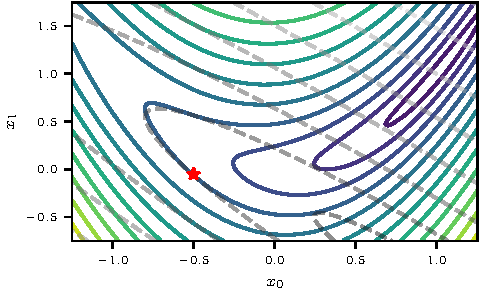
\includegraphics[width=\linewidth]{../kfs/plots/linearized_rosenbrock.pdf}
    \caption{The 2d Rosenbrock function $f_{\alpha=10}$ (solid contour lines) with and its approximation $f'_{\alpha=10, \vx'} = \ell \circ g^{\text{lin}}_{\alpha=10, \vx'}$ (dashed contour lines) when partially linearizing it around an anchor $\vx'$ (star).}
  \end{figure}
\end{example}

\begin{setup}[Composite tensor-to-tensor-to-scalar function]\label{setup:composite_tensor_to_tensor_to_scalar_function}
  Let the tensor-to-scalar function
  \begin{align*}
    f: \sR^{A_1 \times \ldots \times A_N} & \to \sR
    \\
    \tA                                   & \mapsto c = f(\tA)
  \end{align*}
  be the composite of a tensor-to-tensor function $h$ and a tensor-to-scalar function $g$, that is
  \begin{align*}
    f = g \circ h: & \sR^{A_1 \times \ldots \times A_N} \to \sR^{B_1 \times \ldots \times B_M}  \to \sR
    \\
                   & \tA \mapsto \tB = h(\tA) \mapsto c = g(\tB)\,.
  \end{align*}
\end{setup}

\begin{definition}[Generalized Gauss-Newton (GGN) tensor (\Cref{ggns})]\label{def:general_ggn}%
  The GGN tensor of a tensor-to-tensor-to-scalar function $f$ from \Cref{setup:composite_tensor_to_tensor_to_scalar_function}, $\tG_{\tA} f(\tA) \in \sR^{A_1 \times \ldots \times A_N \times A_1 \times \ldots \times A_N}$ is the Hessian of the partially linearized function $\bar{f} = g \circ \lin_{\tA_0}(h)$, evaluated at the anchor point $\tA_0 = \tA$.
  \begin{align*}
    \tG_{\tA} f(\tA)
    =
    \tH_{\tA} \bar{f}(\tA)|_{\tA_0 = \tA}\,.
  \end{align*}
  where $\bar{f} = g \circ \lin_{\tA_0}(h)$.

  We can express this tensor as a tensor contraction between the Jacobians and Hessians of the two composites, \ie 
  \begin{align*}
    [\tG_{\tA} f(\tA)]_{i_1, \ldots, i_N, j_1, \ldots, j_N}
    \\
    =
    \textcolor{VectorPink}{\sum_{k_1, \dots, k_M}}
    \textcolor{VectorBlue}{\sum_{l_1, \dots, l_M}}
     & [\jac_{\tA} \tB]_{\textcolor{VectorPink}{k_1, \dots, k_M}, i_1, \dots, i_N}
    \\
     & [\hess_{\tB} c]_{\textcolor{VectorPink}{k_{1}, \ldots, k_{M}}, \textcolor{VectorBlue}{l_{1}, \ldots, l_{M}}}
    \\
     & [\jac_{\tA} \tB]_{\textcolor{VectorBlue}{l_1, \ldots, l_M}, j_1, \ldots, j_N}\,.
  \end{align*}
\end{definition}
This expression seems daunting at first, so we will convert things back to matrix notation very soon. Before doing that, let's introduce multiplication with the GGN:

\switchcolumn[1]*
\codeblock{basics/ggn_product}
\switchcolumn[0]

\begin{definition}[GGN-vector-product (GGNVP, \Cref{ggn_product})]\label{def:ggnvp}%
  Consider the GGN tensor of a tensor-to-tensor-to-scalar function $f$ from \Cref{setup:composite_tensor_to_tensor_to_scalar_function,def:general_ggn}.
  The GGN-vector-product (GGNVP) $\tU \in \sR^{A_1 \times \ldots \times A_N}$ with a tensor $\tV \in \sR^{A_1 \times \ldots \times A_N}$ from the input domain is
  \begin{align*}
     & [\tU]_{i_1, \dots, i_N}
    \\
     & =
    \sum_{j_1, \dots, j_N}
    [\tG_{\tA} f(\tA)]_{i_1, \dots, i_N, j_1, \dots, j_N}
    [\tV]_{j_1, \dots, j_N}\,,
  \end{align*}
  and decomposes into a JVP, HVP, and JVP when applying the composition from \Cref{def:general_ggn}.
\end{definition}
This is easiest to see for the vector-to-vector-to-scalar case where $\tA, \tB, \tU, \tV \to \va, \vb, \vu, \vv$ and $\vu = (\jac_{\va}\vb)^{\top} (\hess_{\vb} c) (\jac_{\va} \vb) \vv$, which can be written as a matrix chain and computed without explicitly building up any of the matrices in memory~\cite{schraudolph2002fast}.

\paragraph{Matricization} As for the Hessian and Jacobian, we can flatten both composite functions before applying the partial linearization and taking the Hessian to obtain the GGN.
This is equivalent to matricizing the GGN tensor from \Cref{def:general_ggn}.
And it is also equivalent to matricizing the Hessians and Jacobians in the general definition.

\begin{definition}[$\cvec$ and $\rvec$ GGN matrices, \Cref{ggns}]\label{def:vec_ggns}
  For a tensor-to-tensor-to-scalar function $f$ from \Cref{setup:composite_tensor_to_tensor_to_scalar_function}, we define the $\cvec$ and $\rvec$ GGN matrices by flattening the composite functions before applying the partial linearization and taking the Hessian. This yields the flattened GGN matrices $\ggn^{\vec}_{\tA}f(\tA) \in \sR^{A_1 \cdots A_N \times A_1 \cdots A_N}$ where $\vec \in \{\cvec, \rvec\}$ which can be written as matrix chain
  \begin{align*}
    \ggn^{\vec}_{\tA} f(\tA)
    =
    (\jac^{\vec}_{\tA} \tB)^{\top}
    (\hess^{\vec}_{\tB} c)
    (\jac^{\vec}_{\tA} \tB)\,.
  \end{align*}
  using the previously defined flattened Hessians (\Cref{def:cvec_hessian,def:cvec_hessian}) and Jacobians (\Cref{def:cvec_jacobian,def:rvec_jacobian}).
\end{definition}

Again, it is important to emphasize that the matrix GGN depends on the flattening scheme.
To emphasize this point, we conclude this section with the following:

\switchcolumn[1]*
\codeblock{basics/ggns_linear_regression}
\switchcolumn[0]

\begin{example}[GGN of linear regression (\Cref{ggns_linear_regression})]
  Consider the least squares objective
  \begin{align*}
    \gL(\mW) = \sum_n \ell_n(\mW)
  \end{align*}
  where $\ell_n = c_n \circ f_n$ is the composition of a linear classifier and square loss
  on a data point labeled $n$, that is
  $f_n(\mW) = \mW \vx_n$ and $c_n(\vz) = \frac{1}{2}\left\lVert \vz - \vy_n \right\rVert^2_2$.

  Using the shorthands $\vf_n \coloneq f_n(\mW)$ and $c_n \coloneq c_n(\vf_n)$, the matrix GGNs are given by
  \begin{align*}
    \ggn_{\mW}^{\vec}\gL(\mW)
    \coloneq
    \sum_n
    \ggn_{\mW}^{\vec} \ell_n(\mW)
    \\
    =
    \sum_n
    (\jac^{\vec}_{\mW} \vf_n)^{\top}
    (\hess^{\vec}_{\vf_n} c_n)
    (\jac^{\vec}_{\mW} \vf_n)\,.
  \end{align*}
  We can use the results from previous examples, specifically \Cref{jacobians_linear_layer,ex:square_loss_hessian}, to obtain the following expressions
  \begin{align*}
    \ggn_{\mW}^{\cvec}\gL(\mW)
     & =
    \left(
    \sum_n \vx_n \vx_n^{\top}
    \right)
    \otimes \mI
    \\
    \ggn_{\mW}^{\rvec}\gL(\mW)
     & =
    \mI
    \otimes
    \left(
    \sum_n \vx_n \vx_n^{\top}
    \right)
  \end{align*}
\end{example}
Two interesting observations about this result are (i) both GGNs are a Kronecker product (ii) whose order of factors depends on the flattening scheme we are using.
This already hints at using a Kronecker product to approximate the exact GGN, which is what KFAC aims to do.


%%% Local Variables:
%%% mode: latex
%%% TeX-master: "../main"
%%% End:


\switchcolumn[0]*
\subsection{Curvature Matrices in Deep Learning}
\subsubsection{The Hessian}

\subsubsection{The Generalized Gauss-Newton (GGN)}
Linearization

\subsubsection{The Fisher}
Probabilistic perspective

Explain type-1 versus type-2
\subsubsection{The Connection between GGN \& Fisher}
\subsubsection{The Empirical Fisher (EF)}

%%% Local Variables:
%%% mode: latex
%%% TeX-master: "../main"
%%% End:
